\documentclass[12pt,a4paper,twoside,openright]{book}

\usepackage[a4paper,left=2.8cm,right=2.8cm,top=2.8cm,bottom=2.8cm]{geometry}
%\documentclass[paper=a4, fontsize=11pt]{scrartcl} % A4 paper and 11pt font size

\usepackage[T1]{fontenc} % Use 8-bit encoding that has 256 glyphs
%\usepackage{fourier} % Use the Adobe Utopia font for the document - comment this line to return to the LaTeX default
\usepackage[english]{babel} % English language/hyphenation
\usepackage[utf8]{inputenc}  %allows non-English characters
\usepackage{amsmath,amsfonts,amsthm, amssymb, mathrsfs} % Math packages
\usepackage{float}


\usepackage{indentfirst}
\usepackage{caption}
\usepackage{subcaption}
\usepackage{tocbibind}

\usepackage{verbatim}
\usepackage{titlesec}
\usepackage{longtable}
\usepackage{listings}
\usepackage{fancyvrb}
\fvset{frame=single,framesep=1mm,commandchars=\\\{\}}
\usepackage[pdftex]{hyperref,color,graphicx}
%\usepackage[pdftex]{hyperref}
\usepackage{import}
%\usepackage[pdftex,bookmarks,colorlinks]{hyperref}
\usepackage{url}
\usepackage[usenames,dvipsnames]{xcolor}
\usepackage{rotating}
\usepackage{colortbl}
\usepackage{array}
\usepackage[Conny]{fncychap}
\usepackage{listings}
\usepackage{caption}
\renewcommand{\lstlistingname}{Code}
\makeatletter
\renewcommand{\DOCH}{%
    \vskip -4.5\baselineskip
    \mghrulefill{3\RW}\par\nobreak
    %\vskip -0.5\baselineskip
    \mghrulefill{\RW}\par\nobreak
    \CNV\FmN{\@chapapp}\space \CNoV\thechapter
    \par\nobreak
    \vskip -0.5\baselineskip
   }
  \renewcommand{\DOTI}[1]{%
    \mghrulefill{\RW}\par\nobreak
    \CTV\FmTi{#1}\par\nobreak
    \vskip 30\p@
    }
  \renewcommand{\DOTIS}[1]{%
    \mghrulefill{\RW}\par\nobreak
    \CTV\FmTi{#1}\par\nobreak
    \vskip 60\p@
    }
\makeatother

% subfigure and wrapping on figures
\usepackage{subcaption}
\usepackage{wrapfig}

\usepackage[intoc]{nomencl}
\makenomenclature

\hypersetup{
pdftitle={Anonymous Threshold Signatures},
pdfauthor={Hlad Colic, Petar},
%pdfsubject={},
%pdfkeywords={},
colorlinks,
linkcolor=black,
citecolor=black,
urlcolor=blue,
unicode=false
}

\usepackage{fancyhdr} % Custom headers and footers
\pagestyle{fancyplain} % Makes all pages in the document conform to the custom headers and footers
\renewcommand{\sectionmark}[1]{\markright{\thesection\ #1}}
\fancyfoot[LE,RO]{\thepage}
\fancyfoot[C]{}
\fancyhead[RO]{\footnotesize\bfseries}
\fancyhead[LE]{\footnotesize\bfseries}
%\fancyhead[LO,RE]{}

\setcounter{secnumdepth}{4} 
\graphicspath{{../figs/}}

%Include degree symbol in plain text
\usepackage{gensymb}


%Notes on the page (toggle last lines)
\usepackage[colorinlistoftodos]{todonotes}
\setlength{\marginparwidth}{2cm}
\newcommand{\mytodo}[1]{\todo[size=\footnotesize]{#1}}

%\usepackage{biblatex}
\usepackage{enumitem}

\usepackage{flafter}
\usepackage{multirow}
\newcolumntype{M}[1]{>{\arraybackslash}p{#1}}
\newcolumntype{N}{@{}m{0pt}@{}}
\usepackage{pbox}
\usepackage[gen]{eurosym}
%\newcommand{\euro}{euroWARNING}

\lstdefinestyle{tt}{
breakatwhitespace=true,
breaklines     = true,
  frame=top,frame=bottom,
  basicstyle=\small\normalfont\sffamily,    % the size of the fonts that are used for the code
   stepnumber=1,
   numbersep=10pt,                     % how far the line-numbers are from the code
   numbers=left,
   numberstyle=\tiny\color{gray},
  tabsize=2,                              % tab size in blank spaces                     %
  breaklines=true,                        % sets automatic line breaking
  captionpos=t,                           % sets the caption-position to top
    showspaces=false,           % Leerzeichen anzeigen ?
  showtabs=false,             % Tabs anzeigen ?
  xleftmargin=17pt,
  framexleftmargin=17pt,
  framexrightmargin=17pt,
  framexbottommargin=5pt,
  framextopmargin=5pt,
  showstringspaces=false
 }
\DeclareCaptionFormat{listing}{#1#2#3}
\captionsetup[lstlisting]{format=listing,singlelinecheck=false, margin=0pt, font={sf}}

\usepackage{adjustbox}

\usepackage{pdfpages}
\usepackage{afterpage}

%shortcuts for typing variance and expectation
\newcommand{\E}{\mathrm{E}}
\newcommand{\Var}{\mathrm{Var}}
\newcommand{\RR}{{\mathbb R}}
\newcommand{\ZZ}{{\mathbb Z}}
\newcommand{\PP}{{\mathcal P}}
\newcommand{\A}{{\mathcal A}}
\newcommand{\con}{\! \parallel \!}

\theoremstyle{plain}
\newtheorem{thm}{Theorem}[section]
\newtheorem{cor}[thm]{Corollary}
\newtheorem{prop}[thm]{Proposition}

\theoremstyle{definition}
\newtheorem{prob}[thm]{Problem}
\newtheorem{defn}[thm]{Definition} 
\newtheorem{exmp}[thm]{Example}
\newtheorem{remk}[thm]{Remark}

\usepackage[backend=bibtex, style=alphabetic, maxnames=4, minnames=3, maxbibnames=99]{biblatex}

\bibliography{parts/bibliography.bib}
\usepackage{pdfpages}
%%%%%%%%%%%%%%%%%%%%%%%%%%%%%%%%%%%%%%%%
\begin{document}
\newcommand{\titol}{Anonymous threshold signatures}
\newcommand{\shortitol}{Anonymous threshold signatures}
\newcommand{\autor}{Petar Hlad Colic}

% PÀGINA INICIAL
\frontmatter


\includepdf[pages=-]{parts/portada.pdf}
\clearpage{\thispagestyle{empty}\cleardoublepage}
%\pagenumbering{Roman}
\begin{titlepage}
   	
\includegraphics[scale=1]{images/logoUPC.jpg}
   	\hfill
   	
\includegraphics[scale=0.6]{images/logoFME.jpg}\\

   	\begin{center}
   	\vspace{1em}
   	\LARGE\textbf{\MakeUppercase{\titol}} \\
   	\vspace{2em}
   	\large\textit{\textbf{A master's thesis}}\\
   	\large\textit{\textbf{Submitted to the}}\\
   	\vspace{0.5em}
   	\Large\textbf{Facultat de Matem\`atiques i Estad\'istica}\\
   	\vspace{0.5em}
   	\Large\textbf{Universitat Politècnica de Catalunya}\\
   	\vspace{1em}
   	\large\textit{\textbf{By}}\\
   	\LARGE\textbf{\autor}\\
   	\vspace{2em}
   	\large\textit{\textbf{In partial fulfillment}}\\
   	\large\textit{\textbf{of the requirements for the master's degree in}}\\
   	\vspace{0.5em}
   	\Large\textbf{Advanced Mathematics and Mathematical Engineering}\\
   	\vspace{4em}
   	\Large\textbf{Advisor: Javier Herranz Sotoca}\\
   	\vspace{3em}
   	\large\textbf{Barcelona, June 2018}\\
   	\end{center}
\end{titlepage} 
%\pagestyle{plain}
\clearpage{\thispagestyle{empty}\cleardoublepage}
%ABSTRACT
%\thispagestyle{plain}
%\addcontentsline{toc}{section}{Abstract}
\section*{Abstract}

The goal of this work was to find an anoymous threshold signature scheme with compact signature. Although such scheme is not found in this work, few solutions published by other authors are reviewed and an improvement is proposed to obtain a scheme similar to the desired one computationaly expensive and interactive

\section*{Resum}

Aquest treball tenia l'objectiu de trobar un esquema de llindar de signatura an\`onima compacte. Tot i no haver-ne trobat cap, s'analitzen diverses solucions que s'acosten a l'objectiu publicades per altres autors i es proposa una millora per obtenir un esquema com el desitjat costós i interactiu.

\section*{Resumen}

Este trabajo tenía el objetivo de encontrar un esquema umbral de firma anónima compacta. Aún no haberla encontrado, se analizan diversas soluciones que se acercan al objetivo publicadas por otros autores y se propone una mejora para obtener un esquema como el deseado costoso e interactivo.
\clearpage{\thispagestyle{empty}\cleardoublepage}

%% Discomment for "thanks" page.
%\thispagestyle{plain}
%\phantom{aaa}
\vspace{6em}\
\begin{flushright}
	\textit{
	``Agraïments''\\
	Autor Frase
	}
\end{flushright}

%\newpage{\cleardoublepage}

%% Acknowledgements
%\thispagestyle{plain}
%\addcontentsline{toc}{section}{Acknowledgements}
\clearpage{\thispagestyle{empty}\cleardoublepage}
\chapter*{Acknowledgements}

\noindent
Special thanks to my advisor Javier, for his help and patience.

\noindent
And to Ari, for her support.
\clearpage{\thispagestyle{empty}\cleardoublepage}
{\tableofcontents
\clearpage{\thispagestyle{empty}\cleardoublepage}

% To force the figures to appear:
\setcounter{tocdepth}{2}
%\addcontentsline{toc}{section}{List of Figures}
\setcounter{tocdepth}{2}
\listoffigures
\clearpage{\thispagestyle{empty}\cleardoublepage}

%\addcontentsline{toc}{section}{List of Tables}
%\newpage\null\thispagestyle{empty}\newpage
\listoftables
\clearpage{\thispagestyle{empty}\cleardoublepage}
%\thispagestyle{plain}
%\addcontentsline{toc}{section}{Nomenclature}
%\printnomenclature
%\newpage{\cleardoublepage}

\clearpage
\pagestyle{fancy}
\setlength{\parskip}{3mm plus1mm minus1.5mm}
%\thispagestyle{empty}
%\pagenumbering{arabic}
\mainmatter
\chapter{Introduction}

\cite{Phillips1992}
\cite{BlSt97}

An access structure $\Gamma$ is the set of all subsets of $\PP$ that can recover the secret.

\defn Let $\PP := \{ P_1, \dots, P_n \}$ be a set of participants. A \textit{monotone access structure} $\Gamma$ on $\PP$ is a subset $\Gamma \subseteq 2^{\PP}$, such that $$ A \in \Gamma, \quad A \subseteq A' \subseteq \PP \Rightarrow A' \in \Gamma $$

\defn Let $\PP := \{ P_1, \dots, P_n \}$ be a set of participants and let $A \subseteq 2^{\PP}$. The \textit{closure} of $A$, denoted $\cl (A)$, is the set $$ \cl (A) = \{ C: \exists B \in A \text{ s.t. } B \subseteq C \subseteq \PP \}$$

For a monotone access structure $\Gamma$ we have $\Gamma = \cl (\Gamma)$.

\defn Let $\Gamma$ be an access structure on a set of participants $\PP$. $B \in \Gamma$ is a \textit{minimal} qualified set if $A \notin \Gamma$ whenever $A \subsetneq B$.

\defn Let $\Gamma$ be an access structure on a set of participants $\PP$. The family of minimal qualified sets $\Gamma_{0}$ of $\Gamma$ is called a \textit{basis} of $\Gamma$.

For a basis $\Gamma_0$ of an access structure $\Gamma$ we have $\Gamma = \cl (\Gamma_{0})$

\defn An access structure $\Gamma$ is \textit{trivial} if either $\Gamma = 2^{\PP}$ or $\Gamma = \{ \PP \}$.

Let $\mathcal{K}$ be a set of $q$ elements called \textit{secret keys}, and let $\mathcal{S}$ be a finite set whose elements are called \textit{shares}. Let $D$ be a \textit{dealer} who wants to share a secret key $\mathbf{k} \in \mathcal{K}$ among the participants in $\PP$. 

\defn A \textit{distribution rule} is a function $f : \PP \cup \{ D \} \rightarrow \KK \cup \SS$ which satisfies the conditions $f(D) \in \KK$ and $f(P_i) \in \SS$ for $i = 1,2, \dots, n$.

Secret sharing schemes will be represented by a collection of distribution rules, which represent a possible distribution of shares to the participants where $f(D)$ is the secret key being shared and $f(P_i)$ is the share given to $P_i$.

\defn Let $\mathscr{F}$ be a family of distribution rules, and let $\mathbf{k} \in \KK$. Then $\mathscr{F}_{\mathbf{k}} := \{ f \in \mathscr{F} : f(F) = \mathbf{k}\}$ is the family of all distribution rules having $\mathbf{k}$ as secret.

If $\kk \in \KK$ is the secret that $D$ wants to share, then $D$ will chose a distribution rule $f \in \F_{\KK}$ uniformly at random.


Let $\{p_{\KK} (\kk) \}_{\kk \in \KK}$ be a probability distribution on $\KK$, and let a collection of distribution rules for secrets in $\KK$ be fixed.

\defn A \textit{perfect secret sharing scheme}, with respect to a monotone access structure $\Gamma \subseteq 2^{\PP}$, is a collection of distribution rules that satisfy the following two properties:
\begin{enumerate}
    \item If a subset $A \in \Gamma$ of participants pool their shares, then they can determine the value of the secret $\kk$.
    \item If a subset $A \notin \Gamma$ of participants pool their shares, then they can determine nothing about the value of the secret $\kk$. Formally, if $A \notin \acc$ then for all $a = \{ (P_i, s_i): P_i \in A \text{ and } s_i \in \SS \}$ with $p(a)>0$, and for all $\kk \in \KK$, it holds $p(\kk \vert a) = p_{\KK}(\kk)$. In other words, the \textit{a priori} probability of the value of $\kk$ does not change after knowing the shares held by $A$.
\end{enumerate}

\defn An \textit{ideal secret sharing scheme} is a secret sharing scheme for which $\vert \KK \vert = \vert \SS \vert$. An access structure admitting an ideal secret sharing scheme will be referred as \textit{ideal access structure}.

\thm Let $\acc$ be an access structure on a set of participants $\PP$. An ideal anonymous secret sharing scheme for $\acc$ exists if and only if either $\acc$ is a $(1,\vert \PP \vert)$ threshold structure, a $(\vert \PP \vert, \vert \PP \vert)$ threshold structure, or the closure of a complete bipartite graph.

\clearpage{\thispagestyle{empty}\cleardoublepage}
\chapter{Preliminaries}

Some cryptographic preliminaries and other definitions.

\newpage

\section{Bilinear pairings}
\cite{DiHe76}

Let $G_1$ and $G_2$ be two (multiplicative) cyclic groups of prime order $q$. Let $g_1$ be a fixed generator of $G_1$ and $g_2$ be a fixed generator of $G_2$.

\defn Computation Diffie-Hellman (CDH) Problem: Given a randomly chosen $g \in G_1$, $g^a$, and $g^b$ (for unknown randomly chosen $a,b \in \ZZ_q$), compute $g^{ab}$.

\defn Decision Diffie-Hellman (CDH) Problem: Given randomly chosen $g \in G_1$, $g^a$, $g^b$, and $g^c$ (for unknown randomly chosen $a,b,c \in \ZZ_q$), decide whether $c = ab$. (If so, $(g, g^a, g^b, g^c)$ is called a valid Diffie-Hellman tuple.)

\defn Computational co-Diffie-Hellman (co-CDH) Problem on $(G_1, G_2)$: Given $g_2, g^a_2 \in G_2$ and $h \in G_1$ as input, compute $h^a \in G_1$.

\defn Decision co-Diffie-Hellman (co-DDH) on $(G_1, G_2)$: Given $g_2, g^a_2 \in G_2$ and $h, h^b \in G_1$ as input, decide whether $a=b$. If so, we say that $(g_2, g^a_2, h, h^a)$ is a co-Diffie-Hellman tuple.

\defn Bilinear map: Let $G_T$ be an additional group such that $ |G_1| = |G_2| = |G_T| $. A bilinear map is a map $e: G_1 \times G_2 \rightarrow G_T$ with the following properties:
\begin{enumerate}

\item Bilinear: for all $u \in G_1, v \in G_2$ and $a,b \in \ZZ$, $e(u^a, v^b) = e(u,v)^{ab}$.
\item Non-degenerate: $e(g_1, g_2) \neq 1$.

\end{enumerate}

\defn A gap group is a group on which the DDH problem is easy but the CDH is hard.

\newpage

\section{Homomorphic PKE}

\section{Digital Signatures}
To ensure integrity of data in communications and authentication, the concept of digital signatures was developed. 

A digital signature scheme consists of 3 algorithms:
\begin{itemize}
    \item \textbf{Key generation}: on input of a security parameter $k$ (usually the length), outputs a pair $(sk, pk)$ of secret and public keys.
    \item \textbf{Signature}: given an input message $m$ and the secret key $sk$, outputs a signature $\sigma$.
    \item \textbf{Verification}: given an input message $m$, a signature $\sigma$ on the message and a public key $pk$, ouptuts whether the signature is valid or not.
\end{itemize}

A signature scheme must satisfy the following properties:
\begin{itemize}
    \item \textbf{Correctness}: A signature generated with the signing algorithm must always be accepted by the verifier.
    \item \textbf{Unforgeability}: Only a user can sign messages on behalf of himself.
    \item \textbf{Non-repudiation}: 
\end{itemize}

\subsection{Examples}
\subsubsection{ElGamal}
Let $H$ be a collision-resistant hash function. Let $p$ be a large prime such that the \textit{discrete logarithm problem} is difficult over $\ZZ_p$. Let $g$ be a randomly chosen generator of $\ZZ_p^\ast$

\paragraph{Key Generation}

Randomly choose a secret key $x \in \ZZ_p^\ast$, and compute the public key $y = g^x$.

\paragraph{Signature}

To sign a message $m$, the signer chooses a random $k \in \ZZ_p^\ast$.
Compute $ r = g^k$. To compute $s$, the following equation must be satisfied: $g^{H(m)} = g^{xr} g^{ks}$.
So $s = \left( H(m) - xr \right) k^{-1} \quad (\text{mod } p-1)$

If $s=0$, it starts over again with a different $k$.

The pair $(r,s)$ is the digital signature for $m$.

\paragraph{Verification}

Check $g^{H(m)} = y^r r^s$

The use of $H( \cdot )$ prevents an existential forgery attack.

\subsubsection{Boneh-Lynn-Shacham (BLS)}
\cite{BonehLS01}
Let $G,G_T$ be (¿gap?) groups of prime order $p$. Let $g$ be a generator of $G$. Let $e:G \times G \rightarrow G_T$ be a non-degenerate bilinear pairing.
\paragraph{Key Generation}

Randomly choose a secret key $x \in \ZZ_p$. The public key will be $y = g^x$.

\paragraph{Signature}

The signature on $m$ is $\sigma = H(m)^x$.

\paragraph{Verification}

Given a signature $\sigma$ and a public key $g^x$, it verifies that $e(\sigma,g) = e \left( H(m), g^x \right)$.

\section{Signature Aggregation}
Explain how different signature schemes allow aggregation of n signatures on n messages from n signers.

\newpage
\section{Group Signatures}
Use of aggregation: group signatures. They are used to sign on behalf of the group, prove group membership.

The easyest way is to give everyone the secret key, so they can sign. But this would let any colluded user to share the secret key to other parties, which is not admissible.

Some group signatures need what is called a Dealer, which will deal with the keys.

Examples of Group signatures:

\section{Shamir Secret Sharing}
Shamir secret sharing described in \cite{Sham79}.

The scheme is based on polynomial interpolation.

Let $p$ be a large prime number. All operations are done in $\ZZ_p$

We want to share a secret $s$ into $n$ shares so that the secret can be recovered with any $k$ distinct shares.

Let $q(x) = a_0 + a_1 x + \cdots + a_{k-1} x^{k-1}$ be a random polynomial of degree $k-1$ in which $a_0 = s$.

Each participant $i$ in $\PP = \{ 1, ... , n \}$ is given a different random number $x_i \in \ZZ_p$ which identifies the participant.
Then, each participant $i$ is given the share $y_i = q(x_i)$.

To recover the secret, we only need $k$ different shares. Let $P \subset \PP$ be any subset of $k$ participants. Then

Let $\lambda_i^{P} = \prod_{P_j \in (P \setminus P_i)} \frac{-x_j}{x_i - x_j}$

$$
    q(x) = \sum_{i \in P} y_i \prod_{\substack{j \in P \\ i \neq j}} \frac{x-x_j}{x_i-x_j}
$$

Then, $s = q(0)$.

\section{Threshold signature scheme using Shamir}
\label{sec:shamir_sig}

This signature scheme will be based on the BLS scheme.

Let $G$ be a gap group of some prime order $p$. Let $g \in G$ be a generator of the group.

Let $\mathcal{P}= \{ 1, \dots , n \}$ be the set of participants in this scheme. Supose every participant $P_i \in \mathcal{P}$ is given a distinct random number $x_i \in \ZZ_p$ as in the Shamir Secret Sharing Scheme.

Let $SK \in \ZZ_p$ be the secret key of the scheme. Let $q(x) = \sum_{i=0}^{k-1} a_i x^i$ be a random polynomial of degree $k-1$ but fixing $a_0 = SK$.

Each participant $P_i$ is given the share $s_i = q(x_i)$.

So $$SK = \sum_{i \in P} s_i \lambda_i^P$$

To sign a message $m$, each participant $P_i$ computes his partial signature $\sigma_i (m) = H(m)^{s_i}$ and broadcasts de pair $(x_i, \ \sigma_i (m))$.

Then, after a set $P$ of at least $t$ participants has broadcast their partial signatures for the message, a standard signature $\sigma$ can be computed:

$$ \sigma (m) = \prod_{P_i \in P} \sigma_i (m)^{\lambda_i^{P}}= H(m)^{\sum_{P_i \in P} \lambda_i^P s_i} = H(m)^{SK}$$

The signature is valid if $e(\sigma, g) = e(H(m), PK)$

\section{Anonymity}
The concept of anonimity is used in so many ways

You could use ring signatures which proofs the knowledge of a 1-out-of-N secret key. This could be useful for a small amount of signatures. But it is not useful to provide general anonymity.

A signature scheme provides anonymity if:
\begin{itemize}
    \item Unlinkability: cannot decide whether two different signatures were signed by the same user.
    \item Untraceability: cannot get the public key of the signer from a valid signature.
\end{itemize}
\clearpage{\thispagestyle{empty}\cleardoublepage}
\chapter{Single use: Anonymity}
\label{chap:single}
In this chapter we consider threshold signature schemes with non-traceability but with linkability.

As we commented previously, we can avoid the linkability of a threshold signature scheme by setting it up newly every time a signature is computed. We describe two examples.

\section{Anonymous Secret Sharing Scheme}
Consider a signature scheme with secret $sk$. Using the $(t,n)$-anonymous threshold secret sharing scheme described in \cite{BlSt97} we can share the secret $sk$ among the participants through a secure channel. When a set of $t$ participants want to sign a message, they can just recover the secret $sk$ and compute a signature with it.

After that, the signature scheme is newly setup by choosing a different secret $sk$ and sharing it again using an anonymous threshold secret sharing scheme.

In this solution, the dealer (the one who gives the shares to the participants) can know which participant holds which share because the participants have to authenticate themselves to avoid a single participant getting multiple shares. We can approach this by running a $1$-out-of-$N$ OT protocol randomly choosing a share for sufficiently large $N \gg n$ s.t. the probability of two participants choosing the same share is sufficiently low. In this way, the dealer does not know which participants holds which share, but the execution of an OT protocol for large $N$ is computationaly way too expensive.

A solution in this way for the e-voting case described in the introduction would be the following:
\begin{itemize}[align = left, leftmargin=*, label={--}]
\item Let $C_1, ..., C_k$ be the candidates to be voted, and let $\{P_1, ..., P_n\}$ be the set of voters. Each candidate needs at least $t$ votes to be validated. A voter can vote more than one candidate.
\item Let $p$ be a sufficiently large prime. For each $C_i$, the system chooses a random secret $sk_i \in_R \ZZ_p$ and a random polynomial $Q_i(x) = \sum_{j=0}^{t-1} a_{i,j} x^j$ of degree $t-1$ where $a_{i,0} = sk_i$.
\item Each candidate $P_j$ chooses $k$ random values $\alpha_{j,1}, ..., \alpha_{j,k} \in_R \ZZ_p$, then runs an oblivious polynomial evaluation protocol to learn the evaluations $Q_1(\alpha_{j,1}), ..., Q_k(\alpha_{j,k})$ from the system.
\item If a voter $P_j$ wants to vote a candidate $C_i$, just needs to share the pair $(\alpha_{j,i},Q_i(\alpha_{j,i})$.
\item At the end of the voting, if a candidate $C_i$ knows at least $t$ shares $(\alpha_{j,i},Q_i(\alpha_{j,i})$, he can interpolate $Q_i(x)$ to obtain the secret $sk_i = Q_i(0)$ and be validated.
\end{itemize}

\section{Threshold BLS signature}
\label{sec:thr_bls}
Using the BLS threshold signature scheme described in \ref{sec:shamir_sig} we can avoid linkability setting up a new secret after a signature is computed.

After the signature scheme is set up with a new secret $sk$ and a new random polynomial $P(x)$, a participant $P_i$ chooses $\alpha_i \in_R \ZZ_p$ and learns $P(\alpha_i)$ running an oblivious polynomial evaluation protocol. In this way, the dealer does not learn the value of $\alpha_i$.

One could think the following: since the participant actually does not need explicitly the value of $P(\alpha_i)$ but $H(m)^{P(\alpha_i)}$ to compute the partial signature on $m$, the participant can send the exponentiation of the powers of $\alpha_i$ to the dealer ($H(m)^{\alpha_i^j}$ for $j \in \{0, ..., t-1 \}$) and the dealer returns them exponentiated to the coefficients of the polynomial ($\left(H(m)^{\alpha_i^j}\right)^{a_j}$ for $j \in \{0, ..., t-1 \}$). In this way, the participant can compute: $$H(m)^{P(\alpha_i)} = \prod_{0\leq j \leq t-1} \left(H(m)^{\alpha_i^j}\right)^{a_j} = H(m)^{\sum_{0\leq j \leq t-1} a_j \alpha_i^j}$$.

The issue with this last method is that the dealer knows $H(m)^{P(\alpha_i)}$. Then, when the values $\alpha_i$ are published, the dealer can compute the $t^2$ possible partial signatures ${\sigma_{ij} = \left( H(m)^{P(\alpha_i)} \right)^{\lambda_j^P}}$. When the participants publish their partial signatures, the dealer can link them with the value  $H(m)^{P(\alpha_i)}$ and trace their identity.
\clearpage{\thispagestyle{empty}\cleardoublepage}
\chapter{Multiple use: Anonymity with Non-linkability}
\label{chap:mult}
Here we describe three solutions for anonymous threshold signature schemes with non-linkability property.

\section{Constant Size Anonymous Threshold Signature}

\citeauthor*{DazaDSV09} proposed in \cite{DazaDSV09} an anonymous threshold signature scheme that sets a $(t,r)$-threshold signature scheme based on Shamir's secret sharing over a partition of the set $\PP$ of participants.

\subsection{Description}
\label{sec:daza}
\subsubsection*{Setup Algorithm}
\begin{itemize}[align = left, leftmargin=*, label={--}]
\item Let $\PP = \{P_1 , \dots , P_n \}$ be the set of participants. Consider $d$ distinct partitions of $\PP$ into $r$ parts.
$\PP^i = \{\PP^i_1, ... , \PP^i_r\}$ for $i \in \{1, ... , d\}$. This algorithm will set $d$ different threshold signature schemes, one for each partition of $\PP$.

\item Let $p > n$ be a sufficiently large prime. Let $sk_i \in_R \ZZ_p$ be the secret key of the $i$-th threshold signature scheme. Let $P_i(x)$ be a random polynomial over $\ZZ_p$ of degree $t-1$ with ${P_i(0) = \mbox{sk}_i}$ for $i \in \{1, ..., d\}$.

\item For $i \in \{1, ..., d\}$ let $\alpha^{(i)}_1, ... , \alpha^{(i)}_r \in_R \ZZ_p$ all distinct (for fixed $i$). Each participant $P_k \in \PP^i_j$ is given public key $pk^{(i)}_k = \alpha^{(i)}_j$ and secret key $sk^{(i)}_k = P_i(\alpha^{(i)}_j)$ for the $i$-th threshold signature scheme. 
\end{itemize}

\subsubsection*{Signing Algorithm}
\begin{itemize}[align = left, leftmargin=*, label={--}]
\item Let $\{P_{i_1}, ..., P_{i_t} \} \subseteq \PP$ a set of $t$ participants which will try to sign a message $m$.

\item A signature on $m$ over the $i$-th threshold signature scheme is attempted using the protocol described in section \ref{sec:shamir_sig} providing the message, the signature and the signature scheme over which is signed: $(m,\sigma, i)$.

\item If the signature fails (because $\alpha^{(i)}_{i_1}, ... , \alpha^{(i)}_{i_t}$ are not all distinct), a new signature on $m$ is attempted over a threshold signature scheme different from the previous tried.

\item Eventually, the signature will succeed over a certain signature scheme.
\end{itemize}

\subsubsection*{Verifying Algorithm}
\begin{itemize}[align = left, leftmargin=*, label={--}]
\item Let $(m, \sigma, i)$ be a signature on a message $m$. The verification is done using the verifying algorithm described in \ref{sec:shamir_sig}.
\item Let $e$ be a bilinear pairing. The signature is valid if and only if $e(\sigma,g) = e(H(m),pk_i)$.
\end{itemize}

\subsection{Analysis}
In this signature scheme it is not sure that any set of $t$ participants will be able to compute a signature on a given message. The probability of succeeding on signing a message depends on the parameters $t,n,r,d$ and how the partitions are made.

To see the relation between these parameters and the probability of success, we will describe a few examples.

Given $\{P_{i_1}, ... P_{i_t} \}$ a set of $t$ participants, they will succeed only if $\alpha^{(i)}_{i_1}, ..., \alpha^{(i)}_{i_t} $ are all distinct for a certain $i \in \{1, ...,d\}$. Hence, $t \leq r$.

\subsubsection*{Random partitions}
Suppose that for each participant $P_k \in \PP$ and for all $i \in \{1, ..., d\}$ the probability $Pr(P_k \in \PP^i_j) = \frac{1}{r}$ holds.

The probability that, given $t$ participants, they succeed on signing a message in the $i$-th threshold signature scheme (i.e. no two participants share the same public key) is given by $p_{succ,i} = \prod_{k=0}^{t-1} (1-\frac{i}{r}) = 1 - \frac{t(t-1)}{2r} + o\left( \frac{t^2}{r} \right)$

Thus, the probability of failing to sign a message in the $i$-th threshold signature scheme is $p_{fail,i} = 1 - p_{succ,i} = \frac{t^2}{2r} + o\left( \frac{t^2}{r} \right)$.

The global probability of failing to sign a message is $p_{fail} = \prod_{i=1}^d p_{fail,i} = {\left(\frac{t^2}{2r}\right)^d + o\left( \left( \frac{t^{2}}{r} \right)^d \right)}$

\begin{table}[H]
\begin{center}
    \begin{tabular}{|c|r|c|r|r|c|}
        \hline
        $\frac{t^2}{2r}$ & \multicolumn{1}{c|}{$t$} & $\frac{n}{r}$ & \multicolumn{1}{c|}{$n$} & \multicolumn{1}{c|}{$r$} & $p_{fail}$ \\ \hline
        
        \multirow{4}{*}{$10^{-3}$} & $5$ & \multirow{4}{*}{$10^{3}$} & $12.5 \cdot 10^6$ & $12.5 \cdot 10^{3}$ & $0.80 \cdot 10^{-3}$ \\ \cline{2-2} \cline{4-6}
        & $10$ & & $50 \cdot 10^6$ & $50 \cdot 10^{3}$ & $0.90 \cdot 10^{-3}$ \\ \cline{2-2} \cline{4-6}
        & $50$ & & $1.25 \cdot 10^9$ & $1.25 \cdot 10^{6}$ & $0.98 \cdot 10^{-3}$ \\ \cline{2-2} \cline{4-6}
        & $100$ & & $5 \cdot 10^9$ & $5 \cdot 10^{6}$ & $0.99 \cdot 10^{-3}$ \\ \cline{2-2} \cline{4-6}
        
        \hline

    \end{tabular}
\end{center}
\caption{Sample values for $p_{fail,i}$}
\end{table}


\subsubsection*{Deterministic partitions}


To simplify the analysis, for each participant $P_k \in \PP$ we will consider the corresponding codeword in a (not necessary linear) code of length $d$ over an alphabet of size $r$ given by:
$$c_k := (j_1, ... , j_d) \text{ iff } P_k \in \PP^i_{j_i} \quad \forall i \in \{1, ..., d\}$$

\begin{thm}[Singleton \cite{singleton}]
Let $C$ be a code of length $n$, minimum distance $d$ over an alphabet of size $q$ and cardinality $M$. The cardinality is upper bounded by $\log_q M \leq n-d+1$.
\end{thm}

Changing the notation to adapt it to our case, if we want all codewords associated to the participants to be different, we have $log_r n \leq d - \delta + 1$ where $\delta$ would be the minimum distance of the code (i.e. the least number of schemes that any two participants have distinct public keys in them). For $\delta \geq 1$ we have $n \leq r^d$.

It is reasonable to wonder whether it is possible or not to define $d$ partitions of $\PP$, such that any set of $t$ participants lie in different parts of a certain partition $\PP^i$. To answer that question, we need the following definition.

\defn Let $m \geq w \geq 2$. An $(n,m,w)$-perfect hash family is a set of functions $\F$ where $\card{Y} = n$, $\card{X} = m$ and $f: Y \rightarrow X$ for each $f \in \F$, such that, for any $C \subseteq Y$ with $\card{C} = w$, there exists at least one function $f \in \F$ such that $f \vert_C$ is one-to-one. When $\card{\F} = N$, an $(n,m,w)$-perfect hash family will be denoted by \textbf{PHF}$(N;n,m,w)$.

Getting back to our question: let $Y = \PP$, $X = \{1, ..., r\}$ and let $\F = \{f_1, ..., f_d\}$ where $f_i(P_k) = (c_k)_i$. It is possible to define $d$ partitions of $P$ in a way that any set of $t$ participants lie in different parts of a certain partition $P^i$ if and only if there exists a \textbf{PHF}$(d;n,r,t)$. PHF exist only for suitable sets of values for the parameters. The following theorem gives a (not tight) lower bound on $\card{\F}$ s.t. there exists a PHF.

\begin{thm}[2.1 \cite{Deng04}]
There exists a \textbf{PHF}$(d;n,r,t)$ if
$$ d > \frac{\log \binom{n}{t}}{\log r^t - \log (r^t - t! \binom{r}{t})} $$
\end{thm}

\begin{figure}[H]
    \begin{center}
        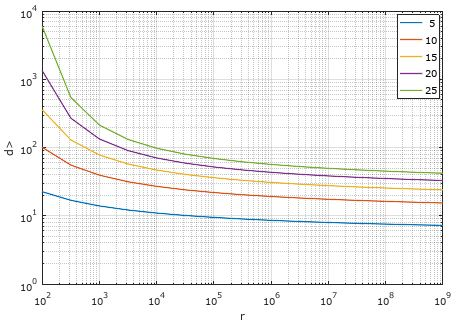
\includegraphics[scale=1.5]{images/phf.jpg}
    \end{center}

    \caption{Lower bound of $d$ for different values of $t$ with $\frac{n}{r} = 10^3$}
    \label{fig:phf} 
\end{figure}

The plot in Figure \ref{fig:phf} gives a hint that the bound might have limit when $r \rightarrow \infty$ fixing $\frac{n}{r}=c$ constant. Note that $r^t - t! \binom{r}{t} = \frac{t(t-1)}{2}r^{t-1} + o(r^{t-1})$ for fixed $t$. Using the inequality $ \left( \frac{n}{t} \right)^t \leq \binom{n}{t} \leq n^t$ and the previous approximation for $r \gg t$, we have:
$$\frac{t \log \frac{n}{t}}{\log r + \log \frac{t(t-1)}{2}} \lesssim \frac{\log \binom{n}{t}}{\log r^t - \log (r^t - t! \binom{r}{t})} \lesssim \frac{t \log n}{\log r + \log \frac{t(t-1)}{2}}$$

Clearly, the limit when $r \rightarrow \infty$ and $n = c \cdot r$ ($c$ a constant), is $t$ on both sides of the inequality.

\section{Linkable Group Signature Scheme}
\label{sec:chen}
\citeauthor{ChenNW11} proposed a $(t,n)$-threshold signature scheme in \cite{ChenNW11} using a group signature scheme where you can link two signatures on the same message but cannot link signatures on different messages. As one can link signatures on the same message, the threshold signature is simply a set of $t$ valid signatures on the same message.
\subsection{Description}
\subsubsection*{Setup Algorithm}
\begin{itemize}[align = left, leftmargin=*, label={--}]
\item Let $G_1$, $G_2$, $G_T$ be cyclic groups of sufficiently large prime order $q$. Two random generators $g_1 \in G_1$, $g_2 \in G_2$, and a bilinear pairing $\hat{t}: G_1 \times G_2 \rightarrow G_T$.

DDH problem in $G_1$, Gap-DL problem in $G_1$ and $G_2$ and the blind bilinear LRSW problem are hard.

\item Let $H_0 : \{0,1\}^\ast \rightarrow \ZZ_q$ and $H_1 : \{ 0 , 1 \}^\ast \rightarrow G_1$ be two hash functions.

\item For each issuer $i \in \mathcal{I}$ the following is performed.

Two integers are selected $x,y \in_R \ZZ_q$ and the issuer secret key \textbf{isk} is assigned to be $(x,y)$. Then the values $X = g_2^{x} \in G_2$ and $Y = g_2^{y} \in G_2$ are computed. The issuer public key \textbf{ipk} is assigned to be $(X,Y)$.

\item The system public parameters $par$ are set to be $par = (G_1, G_2, G_T, \hat{t}, g_1, g_2, H_0, H_1, \text{ipk}_k)$ and are published.
\end{itemize}

\subsubsection*{Join protocol}
\begin{itemize}[align = left, leftmargin=*, label={--}]
\item In this a protocol, an issuer $i \in \mathcal{I}$ computes a credential for a signer $\s \in S$ that allows him to compute valid signatures on messages.

\item The signer $\s$ randomly chooses the secret key $sk_\s = f \in_R \ZZ_p$ and computes the public key $pk_\s = F = g_1^f$.

\item The issuer $\i$ randomly chooses $r \in_R \ZZ_q$ and computes $A = g_1^r$, $B = A^y$ and ${C = A^x F^{rxy}}$. The credential for $\s$ is set to be $cre_\s \leftarrow (A,B,C)$.
\end{itemize}

%\begin{figure}[H]
%$$
%\begin{array}{ccc}
%    \text{Signer}(\mathfrak{s}) &    & \text{Issuer}(\mathfrak{i}) \\
%    \hline
%    \\
%    f \in_R \ZZ_q, \ F = g_1^f &    &    \\
%    \text{str} \leftarrow X \parallel Y \parallel n_I &  \xleftarrow{\text{comm}_{\text{req}}} & \text{comm}_{\text{req}} \leftarrow n_I \\
%        & \longrightarrow & \text{If } F = g_1^{f_i} \text{ for any } f_i \text{ on the roge list then \textbf{abort}} \\
%        &        & r\in_R \ZZ_q; \ A = g_1^r; \ B = A^y \\
%    \text{If } \hat{t}(A,Y) \neq \hat{t}(B,g_2) & \xleftarrow{\text{  cre  }} & C = (A^x \cdot F^{rxy}); \ cre \leftarrow(A,B,C) \\
%    \text{or } \hat{t}(A \cdot B^f , X) \neq \hat{t}(C,g_2) &    & \\
%    \text{then \textbf{abort}} &    & \\
%    \hline
%\end{array} 
%$$
%\caption{The Join Protocol}
%\label{fig:join}
%\end{figure}

\subsubsection*{Signing Algorithm}
\begin{itemize}[align = left, leftmargin=*, label={--}]
\item Let $m \in \{0,1\}^\ast$ be the message that a signer $\s$ wants to sign where $sk_\s = f$, $pk_\s = F$ and $cre_\s = (A,B,C)$.

\item $\s$ chooses $z \in_R \ZZ_q$ and computes $J=H_1(m)$, $K = J^f$ and $L = J^z$.

\item $\s$ chooses $a \in_R \ZZ_q$ and randomizes its credential into $(R,S,T) \leftarrow (A^a,B^a,C^a)$, and computes $\tau = \hat{t}(S,X)^z$ where $X$ is from the issuer's public key.

\item $\s$ computes $c \leftarrow H_0(R \con S \con T \con \tau \con J \con K \con L \con m)$ and sets $s = z + c \cdot f$.

\item The signature on $m$ is set to be $\sigma = (R,S,T,J,K,L,c,s)$


\end{itemize}

The computation of $L$,$c$ and $s$ gives a non-interactive Zero-Knowledge Proof of Knowledge for $f$.

The computation of $\tau$ gives a proof of knowledge of the credentials of the signer. This is based on the \textit{Schnorr Signature Scheme} detailed in section \ref{sec:schnorr}.

%\begin{figure}[H]
%$$\begin{array}{l}
%\text{Signer}(\mathfrak{s}) \\
%\hline
%\text{Input: } f \in \ZZ_q; \ n_T \leftarrow \{0,1\}^\ast; \ msg \\
%a \in_R \ZZ_q; \ z \in_R \ZZ_q \\
%J \leftarrow H_1(\text{msgt}); \ K = J^f; \ L = J^z \\
%R = A^a; \ S = B^a; \ T = C^a; \ \tau = \hat{t}(S,X)^z \\
%c \leftarrow H_0(R \parallel S \parallel T \parallel \tau \parallel J \parallel K \parallel L \parallel n_T \parallel \text{msgb}) \\
%s \leftarrow z + c \cdot f \mod q \\
%\sigma \leftarrow (R,S,T,J,K,c,s,n_T) \\
%\text{Output: } \sigma \\
%\hline
%\end{array}
%$$
%\caption{The Sign Algorithm}
%\label{fig:sign}
%\end{figure}

\subsubsection*{Verifying Algorithm}
\begin{itemize}[align = left, leftmargin=*, label={--}]
\item Let $\sigma = (R,S,T,K,L,c,s)$ be a signature on a message $m$ computed by a signer $\s$.

\item The verifier $\v$ checks if $J = H_1(m)$ and $\hat{t}(R,Y) = \hat{t}(S,g_2)$ hold. If not, the signature is not valid.

\item $\v$ computes $\tau ' =  \hat{t}(R,X)^c \hat{t}(S,X)^s \hat{t}(T,g_2)^{-c}$ and $L' = H_1(m)^s \cdot K^{-c}$.

\item The signature is valid only if $c = H_0(R \con S \con T \con \tau' \con K \con L' \con m)$

\end{itemize}


%\begin{figure}[H]
%$$\begin{array}{l}
%\text{Verifier}(\mathfrak{v}) \\
%\hline
%\text{Input: \textbf{ipk}}_k = (X,Y); \ \text{msg} = (\text{msgt}, \text{msgb}) \\
%\sigma = (R,S,T,J,K,c,s,n_T) \\
%\text{If } K = J^{f_i}, \text{ for any } f_i \text{in the set of rogue secret keys, or} \\
%\qquad \hat{t}(R,Y) \neq \hat{t}(S,g_2), \text{ or} \\
%\qquad J \neq H_1(\text{msgt}) \text{ return \textbf{reject}} \\
%\rho_a^\dagger = \hat{t}(R,X); \rho_b^\dagger = \hat{t}(S,X); \rho_c^\dagger = \hat{t}(T,g_2) \\
%\tau^\dagger = (\rho_b^\dagger)^s \cdot (\rho_c^\dagger / \rho_a^\dagger)^{-c} \\
%L^\dagger = J^s \cdot K^{-c} \\
%\text{If } c \neq H_0 (R \con S \con T \con \tau^\dagger \con J \con K \con L^\dagger \con n_T \con \text{msgb}) \text{ return \textbf{reject}} \\
%\text{Otherwise return \textbf{accept}} \\
%\hline
%\end{array}
%$$
%\caption{The Verify Algorithm}
%\label{fig:verify}
%\end{figure}

\subsubsection*{Threshold Checking Algorithm}
\begin{itemize}[align = left, leftmargin=*, label={--}]
\item When a verifier $\v$ receives a signature $(\sigma, m)$, checks that the signature is valid, and then checks the signature against the list of $\ell$ valid signatures $(\sigma_i,m)$ on the message $m$ already received to ensure it is not a duplicate message signed by some verifier. To do it, just check $K \neq K_i$ for $i \in \{1, ..., \ell \}$.

\item If it is not a duplicate, then $\v$ adds $(\sigma, m)$ to the list of valid signatures.

\item When $\ell = t$, the threshold signature is set to be the collection $\{(\sigma_i)\}_{i\in \{1,...,t\}}$ of $t$ valid signatures on $m$ computed by $t$ distinct signers.


\end{itemize}

\section{Anonymous Interactive Protocol}

We propose an interactive protocol based on the signature scheme described in section \ref{sec:shamir_sig}. Recall that this scheme does not have the \textit{unlinkability} property because it uses "pseudonyms" and they are shared to compute the signature. Thus, the idea of this new protocol is to hide these "pseudonyms".

As in the BLS signature scheme, a participant $P_i$ from a subset $P \subset \PP$ of $t$ participants will compute a partial signature $\sigma_i (m)$ on a message $m$. The partial signature will be $\sigma_i (m) = H(m)^{s_i \prod_{P_j \in (P \setminus P_i)} \frac{-\alpha_j}{\alpha_i - \alpha_j}}$.

The goal of this modification is to compute $a^\frac{-\alpha_j}{\alpha_i - \alpha_j}$ without sharing the values of $\alpha_i$ and $\alpha_j$, for $1 \neq a \in G$ and a given $P_j \in P$.

To compute $a^\frac{-\alpha_j}{\alpha_i - \alpha_j}$ we need participants $P_i,P_j$ and a third party $P_s$ that could be any other participant or a reliable party (like secure hardware).

\subsection{Description}
\label{sec:inter}
\subsubsection*{Interaction}
Let $a^{\frac{-\alpha_j}{\alpha_i - \alpha_j}} \leftarrow \mathcal{B}(a,P_i,P_j)$ the protocol that outputs $a^{\frac{-\alpha_j}{\alpha_i - \alpha_j}}$ given $1 \neq a \in G$, a first participant $P_i$ and a second participant $P_j$.

This protocol is split in five steps. In the figures, the arrows between participants represent communication through a secure channel. The $BC$ block represents a broadcast channel, so anything sent to $BC$ is broadcast to the rest. 

\begin{itemize}[align = left, leftmargin=*, label={--}]
\item[\textbf{First step:}] $P_i$ chooses $x_i, x_j, x_s \in \ZZ^*_p$ three random values and shares them with $P_j$ and $P_s$. These will be the new "pseudonyms".

$P_i$ and $P_j$ randomly choose polynomials $f_i, g_i, z_i$ and $f_j, g_j, z_j$, respectively, where: $f_i,f_j$ and $g_i,g_j$ are linear, $g_i(0) = \alpha_i$ and $g_j(0) = \alpha_j$, and $z_i,z_j$ are quadratic polynomials with $z_i(0) = z_j(0) = 0$.

\begin{figure}[H]
        \begin{center}
        \begin{tikzpicture}
            
            \tikzset{vertex/.style = {draw=none,minimum size=1.5em}}
            \tikzset{calc/.style = {rectangle, draw}}
            \tikzset{edge/.style = {->,thick, > = latex'}}
        
            \node[vertex] (Pi) at (0,0) {$P_i$};
            \node[vertex] (Pj) at (4,0) {$P_j$};
            \node[vertex] (Ps) at (2,2.6) {$P_s$};
            \node[vertex] (BC) at (2,1) {BC};
            
            \node[calc] (i) at (-3,-1.5){
                \begin{tabular}{c}
                    $x_i,x_j,x_s \in_R \ZZ_p^{\ast}$ \\
                    $\gamma_{i,0}, \gamma_{i,1}, \gamma_{i,2}, \gamma_{i,3}, \gamma_{i,4} \in_R \ZZ_p$ \\
                    $g_i(x) \leftarrow \gamma_{i,1} \cdot x + \gamma_{i,0}$ \\
                    $f_i(x) \leftarrow \gamma_{i,2} \cdot x + \alpha_i$ \\
                    $z_i(x) \leftarrow \gamma_{i,4} \cdot x + \gamma_{i,3}$
                \end{tabular}
            };
            
            \node[calc] (j) at (7,-1.5){
                \begin{tabular}{c}
                    $\gamma_{j,0}, \gamma_{j,1}, \gamma_{j,2}, \gamma_{j,3} , \gamma_{j,4} \in_R \ZZ_p$ \\
                    $g_j(x) \leftarrow \gamma_{j,1} \cdot x + \gamma_{j,0}$ \\
                    $f_j(x) \leftarrow \gamma_{j,2} \cdot x + \alpha_j$ \\
                    $z_j(x) \leftarrow \gamma_{j,4} \cdot x + \gamma_{j,3}$
                \end{tabular}
            };
            
            \draw[edge] (Pi) to node[sloped,midway,above] {$x_i,x_j,x_s$} (BC);
            
        
        \end{tikzpicture}
        \end{center}

\caption{Step 1}
\end{figure}

\item[\textbf{Second step:}] Let $h(x) = (g_i(x) + g_j(x))(f_i(x) - f_j(x)) + z_i(x) + z_j(x)$. Note that $h(0) = v \cdot (\alpha_i - \alpha_j)$ for $v := g_i(0) + g_j(0)$.

$P_i$ and $P_j$ share with the rest the evaluations of the random polynomials s.t. $P_i,P_j,P_s$ can compute the evaluations $h(x_i),h(x_j),h(x_s)$ respectively.

\begin{figure}[H]
        \begin{center}
        \begin{tikzpicture}
            
            \tikzset{vertex/.style = {draw=none,minimum size=1.5em}}
            \tikzset{calc/.style = {rectangle, draw}}
            \tikzset{edge/.style = {->,thick, > = latex'}}
        
            \node[vertex] (Pi) at (0,0) {$P_i$};
            \node[vertex] (Pj) at (4,0) {$P_j$};
            \node[vertex] (Ps) at (2,2.6) {$P_s$};
            \node[vertex] (BC) at (2,1) {BC};
            
            \node[calc, left = of Pi] (i) { \footnotesize
                \begin{tabular}{c}
                    For $k \in \{i,j,s\}$ \\
                    $g_{ik} \leftarrow g_i(x_k)$ \\
                    $f_{ik} \leftarrow f_i(x_k)$ \\
                    $z_{ik} \leftarrow z_i(x_k)$
                \end{tabular}
            };
            
            \node[calc, right = of Pj] (j) { \footnotesize
                \begin{tabular}{c}
                    For $k \in \{i,j,s\}$ \\
                    $g_{jk} \leftarrow g_j(x_k)$ \\
                    $f_{jk} \leftarrow f_j(x_k)$ \\
                    $z_{jk} \leftarrow z_j(x_k)$
                \end{tabular}
            };
            
            \draw[edge] (Pi) to [bend left=10] node[sloped,midway,above] {$g_{ij},f_{ij},z_{ij}$} (Pj);
            \draw[edge] (Pj) to [bend left=10] node[sloped,midway,below] {$g_{ji},f_{ji},z_{ji}$} (Pi);
            \draw[edge] (Pi) to node[sloped,midway,above] {$g_{is},f_{is},z_{is}$} (Ps);
            \draw[edge] (Pj) to node[sloped,midway,above] {$g_{js},f_{js},z_{js}$} (Ps);
            
        
        \end{tikzpicture}
        \end{center}
\caption{Step 2}
\end{figure}

\item[\textbf{Third step:}] $P_i$,$P_j$,$P_s$ compute the evaluation of $h$ and share it with the rest. $P_i$ and $P_j$ interpolate the value $h(0)$.

\begin{figure}[H]
        \begin{center}
        \begin{tikzpicture}[node distance=0.5cm]
            
            \tikzset{vertex/.style = {draw=none,minimum size=1.5em}}
            \tikzset{calc/.style = {rectangle, draw}}
            \tikzset{edge/.style = {->,thick, > = latex'}}
        
            \node[vertex] (Pi) at (0,0) {$P_i$};
            \node[vertex] (Pj) at (4,0) {$P_j$};
            \node[vertex] (Ps) at (2,2.6) {$P_s$};
            \node[vertex] (BC) at (2,1) {BC};
            
            \node[calc] (i) at (-2.5,-1){ \footnotesize
                \begin{tabular}{c}
                    $h_i \leftarrow (g_{ii} + g_{ji})(f_{ii} - f_{ji}) + z_{ii} + z_{ji}$ \\
                    $h \leftarrow \sum_{k \in \{i,j,s\}} h_k \prod_{\ell \neq k} \frac{- x_\ell}{x_k - x_\ell}$
                \end{tabular}
            };
            
            \node[calc] (j) at (6.5,-1){ \footnotesize
                \begin{tabular}{c}
                    $h_j \leftarrow (g_{ij} + g_{jj}) (f_{ij} - f_{jj}) + z_{ij} + z_{jj}$ \\
                    $h \leftarrow \sum_{k \in \{i,j,s\}} h_k \prod_{\ell \neq k} \frac{- x_\ell}{x_k - x_\ell}$
                \end{tabular}
            };
            
            \node[calc, above = of Ps] (s) { \footnotesize
                \begin{tabular}{c}
                    $h_s \leftarrow (g_{is} + g_{js}) (f_{is} - f_{js}) + z_{is} + z_{js}$
                \end{tabular}
            };
            
            \draw[edge] (Pi) to node[midway,below] {$h_i$} (BC);
            \draw[edge] (Pj) to node[midway,below] {$h_j$} (BC);
            \draw[edge] (Ps) to node[midway,right] {$h_s$} (BC);
            
        
        \end{tikzpicture}
        \end{center}
\caption{Step 3}
\end{figure}

\item[\textbf{Fourth step:}] $P_i$,$P_j$ compute $A_i=a^{\frac{1}{h(0)}(g_i(x_i)+g_j(x_i))}$, $A_j=a^{\frac{1}{h(0)}(g_i(x_j)+g_j(x_j))}$ respectively. $P_j$ shares $A_j$ with $P_i$.

$P_j$ can interpolate the exponents of $A_i$ and $A_j$ and compute $a^{\frac{g_i(0)+g_j(0)}{h(0)}} = a^{\frac{v}{v(\alpha_i - \alpha_j)}} = a^{\frac{1}{\alpha_i-\alpha_j}}$.

\begin{figure}[H]
        \begin{center}
        \begin{tikzpicture}[node distance=0.5cm]
            
            \tikzset{vertex/.style = {draw=none,minimum size=1.5em}}
            \tikzset{calc/.style = {rectangle, draw}}
            \tikzset{edge/.style = {->,thick, > = latex'}}
        
            \node[vertex] (Pi) at (0,0) {$P_i$};
            \node[vertex] (Pj) at (4,0) {$P_j$};
            
            \node[calc, left = of Pi] (i) { \footnotesize
                \begin{tabular}{c}
                    $A_i \leftarrow a^{\frac{1}{h}(g_{ii} + g_{ji})}$ \\
                \end{tabular}
            };
            
            \node[calc, right = of Pj] (j) { \footnotesize
                \begin{tabular}{c}
                    $A_j \leftarrow a^{\frac{1}{h}(g_{ij} + g_{jj})}$ \\
                    $B \leftarrow A_i^{\frac{-x_j}{x_i-x_j}} A_j^{\frac{-x_i}{x_j-x_i}}$
                \end{tabular}
            };
            
            \draw[edge] (Pi) to node[sloped,midway,above] {$A_i$} (Pj);
                        
        
        \end{tikzpicture}
        \end{center}
\caption{Step 4}
\end{figure}

\item[\textbf{Fifth step:}] $P_j$ computes $B^{-\alpha_j} = a^{\frac{-\alpha_j}{\alpha_i - \alpha_j}}$ and shares it with $P_i$. 

\begin{figure}[H]
        \begin{center}
        \begin{tikzpicture}[node distance=0.5cm]
            
            \tikzset{vertex/.style = {draw=none,minimum size=1.5em}}
            \tikzset{calc/.style = {rectangle, draw}}
            \tikzset{edge/.style = {->,thick, > = latex'}}
        
            \node[vertex] (Pi) at (0,0) {$P_i$};
            \node[vertex] (Pj) at (4,0) {$P_j$};
                        
            \node[calc, left = of Pi] (i) { \footnotesize
                \begin{tabular}{c}
                    Output: $B'$
                \end{tabular}
            };
            
            \node[calc, right = of Pj] (j) { \footnotesize
                \begin{tabular}{c}
                    $B' \leftarrow B^{-\alpha_j}$
                \end{tabular}
            };
            
            \draw[edge] (Pj) to node[sloped,midway,above] {$B'$} (Pi);
                        
        
        \end{tikzpicture}
        \end{center}
\caption{Step 5}
\end{figure}
\end{itemize}
\subsubsection*{Partial signature}
Let $P = \{P_i, P_{j_1}, \dots , P_{j_{t-1}} \}$.

For $P_i$ to compute the partial signature over a message $m$, computes $\sigma_i(m) = a_{t-1}$ where $a_k \leftarrow \mathcal{B}(a_{k-1},P_i,P_{j_k})$ for $k \in \{1, ... , t-1 \}$ and $a_0 = H(m)^{s_i}$

$$
\sigma_i (m)
= a_{t-1} {}^{\frac{- \alpha_{j_{t-1}}}{\alpha_{i} - \alpha_{j_{t-1}}}}
= a_k {}^{\frac{- \alpha_{j_{k}}}{\alpha_{i} - \alpha_{j_{k}}} \cdots \frac{- \alpha_{j_{t-1}}}{\alpha_{i} - \alpha_{j_{t-1}}}}
= a_1 {}^{\frac{- \alpha_{j_{1}}}{\alpha_{i} - \alpha_{j_{1}}} \cdots \frac{- \alpha_{j_{t-1}}}{\alpha_{i} - \alpha_{j_{t-1}}}}
= H(m)^{ s_i \frac{- \alpha_{j_{1}}}{\alpha_{i} - \alpha_{j_{1}}} \cdots \frac{- \alpha_{j_{t-1}}}{\alpha_{i} - \alpha_{j_{t-1}}}}
$$

\subsubsection*{Signature}
The signature $\sigma(m)$ on a message $m$ from a group of $t$ participants $\{P_1, ... , P_t \}$ is
$$\sigma(m) = \prod_{i=1}^m \sigma_i(m)$$

\subsection{Analysis}
\subsubsection*{Unlinkability}
The scheme keeps the unlinkability property while all participants remain honest but curious. Consider an interaction step with participants $P_i,P_j,P_s$. If an adversary $\mathcal{A}$ corrupts $P_j$ and $P_s$, $\mathcal{A}$ knows $f_i(x_j)$ and $f_i(x_s)$, being able to interpolate $f_i$ to obtain $\alpha_i = f_i(0)$.

If we want the scheme to be still unlinkable after corrupting $\ell$ participants, we can extend the protocol in an analogous way where $f_k$ and $g_k$ are polynomials of degree $\ell$ and each interaction step needs $2 \ell + 1$ participants ($P_i,P_j$ and $2 \ell - 1$ other parties $P_{s_k}$.

\subsubsection*{Computational Cost}
For a participant $P_i$ to compute $\sigma_i$, $t-1$ interactions with different participants are needed. Then, to compute a valid signature, $t(t-1)$ interactions. We can consider this computationally expensive for large $t$.

\clearpage{\thispagestyle{empty}\cleardoublepage}
\chapter{Conclusions and future work}
\label{chap:conc}
In this chapter we sum up the advantages and disatvantages of the solutions discussed in chapters \ref{chap:single} and \ref{chap:mult}.

The protocols described in \ref{chap:single} are anonymous and unlinkable, but they are not practical in many applications, since the whole system has to be set up again after a signature is computed.

The signature scheme described in section \ref{sec:daza} simulates a $(t,n)$-threshold signature scheme setting $d$ different $(t,r)$-threshold signature schemes. Not always a group of $t$ participants can compute a signature.

If we suppose that the participants are homogeneously distributed in the partitions, we can say that the amount of participants in a part $\PP^i_j$ is approximately $g:=\frac{n}{r}$. The unlinkability of the scheme is determined by the value $g$ and must be large enough so that the linkability at the group level does not imply linkability at participant level.

For random partitions, the probability to succeed at signing a message $p \simeq 1 - \frac{t^2}{2r}$ can be improved by setting large $r$, but there is a tradeoff with linkability as $g$ decreases. 

For deterministic partitions there is a smart way set them s.t. any set of $t$ participants can perform a signature. This can be done for sufficiently large $d$. This results in the fact that the participants have to store $d$ key pairs and perform up to $d$ partial signatures to compute a valid signature, and the lower bound on $d$ grows with $t$ and $n$, and decreases with $r$. We have seen that for $r \rightarrow \infty$ with $g \rightarrow c$ then $d \rightarrow t$. Then, we can lower the value of $d$ by increasing $r$. Again, this results in a tradeoff with linkability since $g$ decreases.

An important detail to comment is that to improve the efficiency of the signature for $d \geq 2$ (random or deterministic partitions), the participant could compute the partial signatures for the $d$ schemes, broadcast them, and eventualy one of the $d$ schemes will succeed. But, if no two participants share the same distribution over partitions, this identifies the participants. Thus, in this cases it is likely to avoid this improvement.

The protocol described in section \ref{sec:chen} sets an anonymous $(t,n)$-threshold signature scheme where any set of $t$ participants can compute a signature based on a linkable group signature when signing the same message (but not linkable for signatures on distinct messages). The threshold is achieved by collecting $t$ unlinked signatures over the same message. This implies that the length of the signature grows linearly with $t$ and the verification complexity is quadratic on $t$ (since all $\binom{t}{2}$ pairs of signatures have to be checked).

The protocol described in section \ref{sec:inter} sets an anonymous $(t,n)$-threshold signature scheme that is unlinkable, and untraceable whenever an adversary can corrupt at most one participant. It is compact since the length of the signature is the same as the length of the keys (intependent of $t$). The counterpart is that, since it is interactive, it requires an amount of interactions that is quadratic in $t$. It is a standard BLS signatures and can be verified in constant time (independent of $t$).

The main problem of finding a compact anonymous threshold signature scheme that is unlinkable (or a proof of non-existence) still remains open.

\clearpage{\thispagestyle{empty}\cleardoublepage}
\printbibliography
\addcontentsline{toc}{chapter}{Bibliography}

\end{document}
